\documentclass[12pt,a4paper]{article}

\usepackage[margin=1in]{geometry}
\usepackage{amsmath, amssymb, amsthm}
\usepackage{mathtools}
\usepackage{enumitem}
\usepackage{booktabs}
\usepackage{array}
\usepackage{xcolor}
\usepackage{tikz}
\usetikzlibrary{arrows.meta, positioning}

\setlength{\parindent}{0pt}
\setlength{\parskip}{6pt}

\newtheoremstyle{lecturestyle}
  {8pt}
  {8pt}
  {\normalfont}
  {}
  {\bfseries}
  {.}
  {0.5em}
  {}

\theoremstyle{lecturestyle}
\newtheorem{definition}{Definition}
\newtheorem{example}{Example}
\newtheorem{theorem}{Theorem}
\newtheorem{proposition}{Proposition}
\newtheorem{remark}{Remark}

\newenvironment{answer}
{\par\textbf{Answer.}\ }
{\hfill$\square$\par}

\newcommand{\Prob}{\mathbb{P}}
\newcommand{\E}{\mathbb{E}}

\title{\textbf{Lecture 9: Convergence, Ergodicity, and Applications of Markov Chains}}
\author{MA4034: Time Series and Stochastic Processes}
\date{}

\begin{document}
\maketitle

\section{Review: Stationary Distributions}

From Lecture 8, a probability row vector
\[
\pi=(\pi_i:i\in S)
\]
is called a \textbf{stationary distribution} of a Markov chain with transition matrix $P$ if
\[
\pi P=\pi,
\]
where
\[
\pi_i\geq 0
\qquad\text{and}\qquad
\sum_{i\in S}\pi_i=1.
\]

For an irreducible Markov chain, if a stationary distribution exists, then it is unique. Also, for an irreducible Markov chain, the existence of a stationary distribution is equivalent to positive recurrence.

Thus, if we can find a stationary distribution for an irreducible Markov chain, then we know two important facts:
\begin{itemize}[leftmargin=1.2cm]
    \item the stationary distribution is unique,
    \item the chain is positive recurrent.
\end{itemize}

\section{Convergence to the Stationary Distribution}

In the previous lecture, we studied long-run behaviour using powers of the transition matrix:
\[
P^n.
\]
The natural question is:
\[
\text{Does }P^n\text{ settle down as }n\to\infty?
\]

\begin{definition}[Limit Distribution]
Let $p_{ij}^{(n)}$ be the $n$-step transition probabilities of a Markov chain. If there exists a probability distribution
\[
q=(q_j:j\in S)
\]
such that
\[
p_{ij}^{(n)}\to q_j
\qquad\text{as }n\to\infty
\]
for all $i,j\in S$, then $q$ is called the \textbf{limit distribution} of the Markov chain.
\end{definition}

The important point is that the limit $q_j$ does not depend on the starting state $i$. In the long run, the chain ``forgets'' where it started.

\textbf{Analogy.} Imagine stirring different colours of ink into water. At first, where the ink was dropped matters. After enough stirring, the final colour distribution is the same everywhere. A limit distribution is the Markov chain version of this final mixed state.

\begin{remark}
A stationary distribution and a limit distribution are related, but they are not always the same thing. A stationary distribution can exist even when the limit distribution does not exist. Periodicity is one reason this can happen.
\end{remark}

\section{A Trivial but Important Case: ON/OFF with $p=q=1$}

Consider the ON/OFF chain with states
\[
0=\text{OFF},\qquad 1=\text{ON}.
\]
The general transition matrix is
\[
P=
\begin{pmatrix}
1-p & p\\
q & 1-q
\end{pmatrix}.
\]

When
\[
p=q=1,
\]
the chain always switches to the other state:
\[
P=
\begin{pmatrix}
0 & 1\\
1 & 0
\end{pmatrix}.
\]

\begin{center}
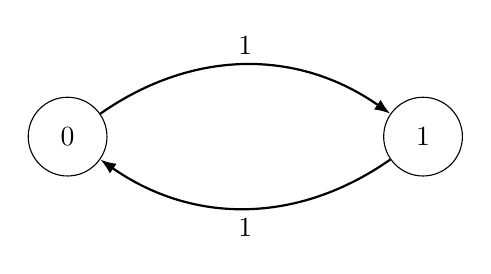
\begin{tikzpicture}[
  state/.style={circle, draw, minimum size=10mm},
  edge/.style={-{Latex[length=2mm]}, thick},
  bend angle=35
]
\node[state] (0) {$0$};
\node[state, right=35mm of 0] (1) {$1$};
\draw[edge] (0) edge[bend left] node[above] {$1$} (1);
\draw[edge] (1) edge[bend left] node[below] {$1$} (0);
\end{tikzpicture}
\end{center}

If the chain starts in state 0, then it is in state 1 after one step, state 0 after two steps, state 1 after three steps, and so on.

\subsection{Stationary Distribution}

Let
\[
\pi=(\pi_0,\pi_1).
\]
The stationary equation is
\[
\pi P=\pi.
\]
Therefore,
\[
(\pi_0,\pi_1)
\begin{pmatrix}
0 & 1\\
1 & 0
\end{pmatrix}
=
(\pi_0,\pi_1).
\]
This gives
\[
\pi_1=\pi_0.
\]
Together with
\[
\pi_0+\pi_1=1,
\]
we get
\[
\pi_0=\pi_1=\frac12.
\]
Hence the stationary distribution is
\[
\boxed{\pi=\left(\frac12,\frac12\right).}
\]

\subsection{No Limit Distribution}

Although the stationary distribution exists, the limit distribution does not exist.

For example,
\[
p_{00}^{(n)}
=
\begin{cases}
1, & n \text{ is even},\\
0, & n \text{ is odd}.
\end{cases}
\]
Thus $p_{00}^{(n)}$ oscillates between 1 and 0. It does not converge.

Therefore,
\[
\lim_{n\to\infty}p_{00}^{(n)}
\]
does not exist, and hence the chain has no limit distribution.

The problem is that the chain is periodic: it returns to state 0 only after an even number of steps.

\section{Periodic and Aperiodic Chains}

\begin{definition}[Period of a State]
The \textbf{period} of a state $i$ is
\[
d(i)=\gcd\{n\geq 1:p_{ii}^{(n)}>0\}.
\]
That is, we look at all possible return times to state $i$ and take their greatest common divisor.
\end{definition}

\begin{definition}[Aperiodic State]
A state $i$ is called \textbf{aperiodic} if
\[
d(i)=1.
\]
\end{definition}

\begin{definition}[Periodic State]
If
\[
d(i)>1,
\]
then state $i$ is called \textbf{periodic}.
\end{definition}

\textbf{Analogy.} A periodic state is like a bus that only arrives every 2 hours, or every 3 hours, in a fixed pattern. An aperiodic state has no strict repeating schedule; returns can happen in a more flexible way.

\begin{example}[ON/OFF Chain with $p=q=1$]
For the chain
\[
P=
\begin{pmatrix}
0 & 1\\
1 & 0
\end{pmatrix},
\]
we have
\[
p_{00}^{(n)}>0
\]
only when $n$ is even. Therefore the possible return times to state 0 are
\[
2,4,6,\ldots
\]
and
\[
d(0)=\gcd\{2,4,6,\ldots\}=2.
\]
Thus state 0 has period 2. Similarly, state 1 also has period 2.
\end{example}

\begin{example}[Aperiodicity in the Gambler's Ruin Type Chain]
Suppose state 1 can return to itself in 2 steps and also in 3 steps. Then
\[
p_{11}^{(2)}>0
\quad\text{and}\quad
p_{11}^{(3)}>0.
\]
Since
\[
\gcd(2,3)=1,
\]
state 1 is aperiodic.

Notice that aperiodic does not mean that a state can return in one step. It only means that the greatest common divisor of the possible return times is 1.
\end{example}

\begin{remark}
Periodicity is a class property. This means that if two states communicate, then they have the same period. Therefore, in an irreducible Markov chain, either all states are periodic with the same period or all states are aperiodic.
\end{remark}

\section{Ergodic Markov Chains}

\begin{definition}[Ergodic Markov Chain]
An irreducible, positive recurrent, and aperiodic Markov chain is called \textbf{ergodic}.
\end{definition}

Ergodicity is exactly the set of conditions needed in the main convergence theorem.

\begin{theorem}[Convergence Theorem for Markov Chains]
Consider an irreducible, positive recurrent, and aperiodic Markov chain with stationary distribution $\pi$ and $n$-step transition probabilities $p_{ij}^{(n)}$. Then
\[
p_{ij}^{(n)}\to \pi_j
\qquad\text{as }n\to\infty
\]
for all $i,j\in S$.
\end{theorem}

In other words, for an ergodic Markov chain, the stationary distribution is also the limit distribution.

\[
\boxed{\text{ergodic} \quad \Longrightarrow \quad \lim_{n\to\infty}P^n
\text{ has every row equal to }\pi.}
\]

\section{Example: Success Runs}

Suppose a fair coin is flipped repeatedly. At time $n$, let $X_n$ be the length of the current run of heads.

For example, if the sequence is
\[
HTHHHT,
\]
and we take $X_0=0$, then
\[
X_1=1,\quad X_2=0,\quad X_3=1,\quad X_4=2,\quad X_5=3,\quad X_6=0.
\]

The state space is
\[
S=\{0,1,2,\ldots\}.
\]

From state $i$:
\begin{itemize}[leftmargin=1.2cm]
    \item if the next toss is heads, the chain moves to $i+1$,
    \item if the next toss is tails, the chain moves back to $0$.
\end{itemize}

Since the coin is fair,
\[
\Prob(\text{heads})=\frac12,
\qquad
\Prob(\text{tails})=\frac12.
\]

Thus
\[
p_{i,i+1}=\frac12,
\qquad
p_{i,0}=\frac12
\]
for every $i\geq0$.

\begin{center}
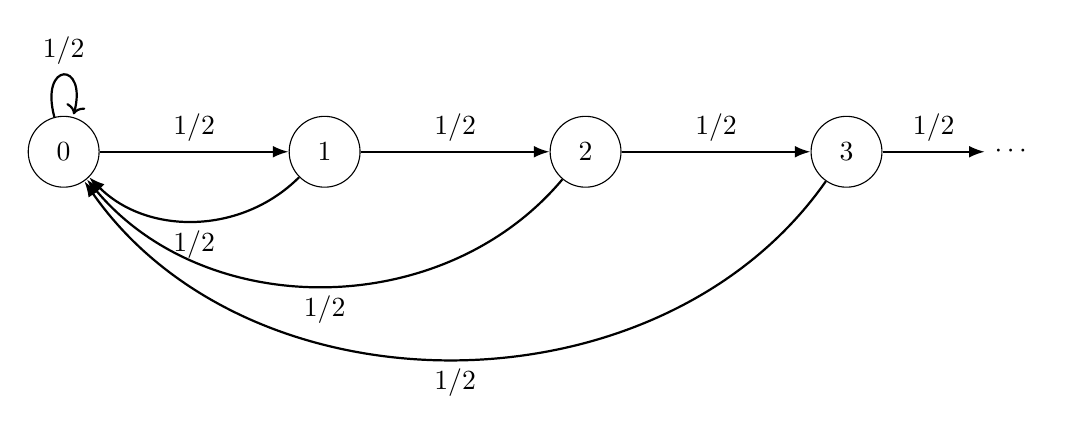
\begin{tikzpicture}[
  state/.style={circle, draw, minimum size=9mm},
  edge/.style={-{Latex[length=2mm]}, thick},
  bend angle=35
]
\node[state] (0) {$0$};
\node[state, right=24mm of 0] (1) {$1$};
\node[state, right=24mm of 1] (2) {$2$};
\node[state, right=24mm of 2] (3) {$3$};
\node[right=13mm of 3] (dots) {$\cdots$};

\draw[edge] (0) edge[loop above] node {$1/2$} (0);
\draw[edge] (0) -- node[above] {$1/2$} (1);
\draw[edge] (1) -- node[above] {$1/2$} (2);
\draw[edge] (2) -- node[above] {$1/2$} (3);
\draw[edge] (3) -- node[above] {$1/2$} (dots);
\draw[edge] (1) edge[bend left=45] node[below] {$1/2$} (0);
\draw[edge] (2) edge[bend left=50] node[below] {$1/2$} (0);
\draw[edge] (3) edge[bend left=55] node[below] {$1/2$} (0);
\end{tikzpicture}
\end{center}

\subsection{Why the Chain is Irreducible}

From any state $i$, a tail takes the chain back to 0. From 0, a sequence of heads can take the chain to any state $j$.

Therefore every state can reach every other state, so the chain is irreducible.

\subsection{Why the Chain is Aperiodic}

State 0 has a self-loop:
\[
p_{00}=\frac12>0.
\]
Thus state 0 can return to itself in one step, so its period is 1. Since the chain is irreducible, all states have the same period. Therefore the whole chain is aperiodic.

\subsection{Stationary Distribution}

Let
\[
\pi=(\pi_0,\pi_1,\pi_2,\ldots).
\]
The stationary equation is
\[
\pi P=\pi.
\]

For $k\geq1$, the only way to enter state $k$ is from state $k-1$ by tossing heads. Hence
\[
\pi_k=\frac12\pi_{k-1}.
\]
Therefore,
\[
\pi_k=\left(\frac12\right)^k\pi_0,
\qquad k=0,1,2,\ldots
\]

Using the condition
\[
\sum_{k=0}^{\infty}\pi_k=1,
\]
we get
\[
1
=
\sum_{k=0}^{\infty}\left(\frac12\right)^k\pi_0
=
\pi_0\sum_{k=0}^{\infty}\left(\frac12\right)^k.
\]
Since
\[
\sum_{k=0}^{\infty}\left(\frac12\right)^k=2,
\]
we have
\[
1=2\pi_0.
\]
Thus
\[
\pi_0=\frac12.
\]
Hence
\[
\pi_k=\left(\frac12\right)^{k+1},
\qquad k=0,1,2,\ldots
\]

So the stationary distribution is
\[
\boxed{
\pi=\left(\frac12,\frac14,\frac18,\frac1{16},\ldots\right).
}
\]

Because the chain is irreducible, positive recurrent, and aperiodic, this is also the limit distribution.

\section{Mean Recurrence and Long-Term Frequency}

For an ergodic Markov chain, the stationary probability $\pi_i$ has an important interpretation:
\[
\pi_i=\text{long-term proportion of time spent in state }i.
\]

Therefore, if $\pi_i$ is large, state $i$ is visited often. If $\pi_i$ is small, state $i$ is visited rarely.

\begin{proposition}[Mean Recurrence Time]
Consider an ergodic Markov chain with stationary distribution $\pi$. Let $\tau_i$ be the return time to state $i$. Then
\[
\E_i[\tau_i]=\frac{1}{\pi_i}.
\]
Also, if $N_j$ is the number of visits to state $j$ between consecutive visits to state $i$, then
\[
\E_i[N_j]=\frac{\pi_j}{\pi_i}.
\]
\end{proposition}

The value
\[
\E_i[\tau_i]=\frac1{\pi_i}
\]
is called the \textbf{mean recurrence time} of state $i$.

\textbf{Analogy.} If a shop receives 1 out of every 10 customers from a certain town, then on average that town appears once every 10 customers. Similarly, if $\pi_i=0.1$, then state $i$ is visited about once every $1/0.1=10$ steps.

\begin{example}[Mean Recurrence in the Biased Gambler's Chain]
Suppose Ann wins with probability
\[
p=\frac13
\]
in the gambler's chain from Lecture 8. The stationary distribution is
\[
\pi_n=
\frac{1-2p}{1-p}
\left(\frac{p}{1-p}\right)^n.
\]
Substituting $p=\frac13$,
\[
\pi_n
=
\frac{1-\frac23}{\frac23}
\left(\frac{\frac13}{\frac23}\right)^n
=
\frac12\left(\frac12\right)^n
=
\frac{1}{2^{n+1}}.
\]

Thus
\[
\pi_0=\frac12,
\qquad
\pi_5=\frac1{64}.
\]

If Ann just went broke, the expected number of rounds until she is broke again is
\[
\E_0[\tau_0]=\frac1{\pi_0}=2.
\]

If Ann reaches a fortune of \$5, the expected number of visits to state 0 before returning to state 5 is
\[
\E_5[N_0]=\frac{\pi_0}{\pi_5}
=
\frac{1/2}{1/64}
=32.
\]
\end{example}

\section{Worked Application 1: Weather Model}

\begin{example}
The weather at a coastal resort is classified each day as either sunny or rainy. A sunny day is followed by another sunny day with probability $0.9$. A rainy day is followed by another rainy day with probability $0.3$.

\begin{enumerate}[label=(\alph*)]
    \item Describe this as a Markov chain.
    \item If Friday is sunny, what is the probability that Sunday is also sunny?
    \item If Friday is sunny, what is the probability that both Saturday and Sunday are sunny?
\end{enumerate}
\end{example}

\begin{answer}
Let
\[
S=\text{sunny},\qquad R=\text{rainy}.
\]
The transition probabilities are:
\[
\Prob(S\to S)=0.9,
\qquad
\Prob(S\to R)=0.1,
\]
\[
\Prob(R\to R)=0.3,
\qquad
\Prob(R\to S)=0.7.
\]

Using the order $(S,R)$, the transition matrix is
\[
P=
\begin{pmatrix}
0.9 & 0.1\\
0.7 & 0.3
\end{pmatrix}.
\]

For part (b), Friday to Sunday is two steps. We need
\[
p_{SS}^{(2)}.
\]
Compute
\[
P^2=
\begin{pmatrix}
0.9 & 0.1\\
0.7 & 0.3
\end{pmatrix}
\begin{pmatrix}
0.9 & 0.1\\
0.7 & 0.3
\end{pmatrix}.
\]
The top-left entry is
\[
p_{SS}^{(2)}
=(0.9)(0.9)+(0.1)(0.7)
=0.81+0.07
=0.88.
\]
Therefore,
\[
\Prob(\text{Sunday sunny}\mid \text{Friday sunny})=0.88.
\]

For part (c), both Saturday and Sunday must be sunny. Thus the path is
\[
S\to S\to S.
\]
Therefore,
\[
\Prob(Saturday=S,Sunday=S\mid Friday=S)
=
(0.9)(0.9)
=0.81.
\]
\end{answer}

\section{Worked Application 2: Finding Transition Probabilities from Joint Probabilities}

\begin{example}
At another resort, it is known that the probability that any two consecutive days are both sunny is $0.7$, and the other three combinations are equally likely. Find the transition probabilities.
\end{example}

\begin{answer}
The four joint probabilities for two consecutive days are
\[
\Prob(S,S)=0.7,
\]
and the other three combinations are equally likely:
\[
\Prob(S,R)=\Prob(R,S)=\Prob(R,R)=0.1.
\]

These are joint probabilities, not transition probabilities.

First find the marginal probabilities:
\[
\Prob(S)=\Prob(S,S)+\Prob(S,R)=0.7+0.1=0.8,
\]
\[
\Prob(R)=\Prob(R,S)+\Prob(R,R)=0.1+0.1=0.2.
\]

Now use conditional probability:
\[
\Prob(S\mid S)=\frac{\Prob(S,S)}{\Prob(S)}
=\frac{0.7}{0.8}
=\frac78,
\]
\[
\Prob(R\mid S)=\frac{\Prob(S,R)}{\Prob(S)}
=\frac{0.1}{0.8}
=\frac18.
\]
Also,
\[
\Prob(S\mid R)=\frac{\Prob(R,S)}{\Prob(R)}
=\frac{0.1}{0.2}
=\frac12,
\]
\[
\Prob(R\mid R)=\frac{\Prob(R,R)}{\Prob(R)}
=\frac{0.1}{0.2}
=\frac12.
\]

Thus, using the order $(S,R)$, the transition matrix is
\[
\boxed{
P=
\begin{pmatrix}
\frac78 & \frac18\\
\frac12 & \frac12
\end{pmatrix}.
}
\]
\end{answer}

\section{Worked Application 3: Defective Components}

\begin{example}
A machine produces electronic components that may be defective or non-defective. Defective components tend to come in clusters. A defective component is followed by another defective component with probability $0.3$, whereas a non-defective component is followed by a defective component with probability $0.01$. Describe this as a Markov chain and find the long-term proportion of defective components.
\end{example}

\begin{answer}
Let
\[
D=\text{defective},\qquad N=\text{non-defective}.
\]
The given probabilities are
\[
\Prob(D\to D)=0.3,
\qquad
\Prob(N\to D)=0.01.
\]
Therefore,
\[
\Prob(D\to N)=0.7,
\qquad
\Prob(N\to N)=0.99.
\]

Using the order $(D,N)$, the transition matrix is
\[
P=
\begin{pmatrix}
0.3 & 0.7\\
0.01 & 0.99
\end{pmatrix}.
\]

Let
\[
\pi=(\pi_D,\pi_N)
\]
be the stationary distribution. We solve
\[
\pi P=\pi,
\qquad
\pi_D+\pi_N=1.
\]

From the first component,
\[
0.3\pi_D+0.01\pi_N=\pi_D.
\]
Hence
\[
0.01\pi_N=0.7\pi_D.
\]
So
\[
\pi_N=70\pi_D.
\]

Using
\[
\pi_D+\pi_N=1,
\]
we get
\[
\pi_D+70\pi_D=1.
\]
Therefore,
\[
71\pi_D=1,
\]
so
\[
\pi_D=\frac1{71}.
\]
Then
\[
\pi_N=\frac{70}{71}.
\]

Thus the stationary distribution is
\[
\boxed{\pi=\left(\frac1{71},\frac{70}{71}\right).}
\]
The long-term proportion of defective components is
\[
\boxed{\frac1{71}\approx 0.0141.}
\]
So, in the long run, about 1 out of every 71 components is defective.
\end{answer}

\section{Worked Application 4: Insurance Risk Categories}

\begin{example}
An insurance company classifies auto insurance policyholders into three categories:
\[
H=\text{high risk},\qquad I=\text{intermediate risk},\qquad L=\text{low risk}.
\]
In any given year, a policyholder has:
\[
\Prob(0\text{ accidents})=0.6,
\]
\[
\Prob(1\text{ accident})=0.2,
\]
\[
\Prob(2\text{ accidents})=0.1,
\]
\[
\Prob(\text{more than 2 accidents})=0.1.
\]
If the policyholder has no accidents, they move down one risk category. If they have one accident, they stay in the same category. If they have two accidents, they move up one risk category. If they have more than two accidents, they move to high risk.

\begin{enumerate}[label=(\alph*)]
    \item Describe the sequence of risk categories as a Markov chain.
    \item If a customer starts as low risk, how many years can they expect to stay there?
    \item How many years pass on average between two consecutive visits to the high-risk category?
\end{enumerate}
\end{example}

\begin{answer}
Use the state order
\[
(H,I,L).
\]

From high risk:
\begin{itemize}[leftmargin=1.2cm]
    \item 0 accidents: move down to intermediate, probability $0.6$,
    \item 1 accident: stay high, probability $0.2$,
    \item 2 accidents: move up, but already high, probability $0.1$,
    \item more than 2 accidents: high, probability $0.1$.
\end{itemize}
Therefore the row for $H$ is
\[
(0.4,0.6,0).
\]

From intermediate risk:
\[
I\to L \text{ with probability }0.6,
\]
\[
I\to I \text{ with probability }0.2,
\]
\[
I\to H \text{ with probability }0.1+0.1=0.2.
\]
So the row for $I$ is
\[
(0.2,0.2,0.6).
\]

From low risk:
\[
L\to L \text{ with probability }0.6+0.2=0.8,
\]
\[
L\to I \text{ with probability }0.1,
\]
\[
L\to H \text{ with probability }0.1.
\]
So the row for $L$ is
\[
(0.1,0.1,0.8).
\]

Thus the transition matrix is
\[
P=
\begin{pmatrix}
0.4 & 0.6 & 0\\
0.2 & 0.2 & 0.6\\
0.1 & 0.1 & 0.8
\end{pmatrix}.
\]

For part (b), if the customer is low risk, they stay low risk in a given year with probability
\[
p_{LL}=0.8.
\]
Therefore the probability of leaving low risk in a given year is
\[
1-0.8=0.2.
\]
The number of years spent in low risk before leaving has a geometric distribution with success probability $0.2$. Hence the expected time is
\[
\frac1{0.2}=5.
\]
So the customer can expect to stay low risk for
\[
\boxed{5\text{ years}}
\]
before moving to another category.

For part (c), we need the mean recurrence time of the high-risk state. First find the stationary distribution
\[
\pi=(\pi_H,\pi_I,\pi_L).
\]
Solving $\pi P=\pi$ and $\pi_H+\pi_I+\pi_L=1$ gives
\[
\pi=\left(\frac5{29},\frac6{29},\frac{18}{29}\right).
\]

Therefore the mean recurrence time for high risk is
\[
\E_H[\tau_H]=\frac1{\pi_H}
=
\frac1{5/29}
=
\frac{29}{5}.
\]
Thus the average time between two consecutive visits to the high-risk category is
\[
\boxed{\frac{29}{5}=5.8\text{ years}.}
\]
\end{answer}

\section{Worked Examples}

\begin{example}[Stationary But Not Limiting]
Show that the chain
\[
P=
\begin{pmatrix}
0 & 1\\
1 & 0
\end{pmatrix}
\]
has a stationary distribution but no limit distribution.
\end{example}

\begin{answer}
Let
\[
\pi=(\pi_0,\pi_1).
\]
The stationary equation is
\[
\pi P=\pi.
\]
Thus
\[
(\pi_0,\pi_1)
\begin{pmatrix}
0 & 1\\
1 & 0
\end{pmatrix}
=
(\pi_1,\pi_0)
=
(\pi_0,\pi_1).
\]
Therefore
\[
\pi_0=\pi_1.
\]
Using
\[
\pi_0+\pi_1=1,
\]
we get
\[
\pi_0=\pi_1=\frac12.
\]
So the stationary distribution is
\[
\pi=\left(\frac12,\frac12\right).
\]

However,
\[
p_{00}^{(n)}
=
\begin{cases}
1, & n\text{ even},\\
0, & n\text{ odd}.
\end{cases}
\]
This sequence does not converge. Therefore the chain has no limit distribution.
\end{answer}

\begin{example}[Finding the Period]
Suppose a state $i$ can return to itself in 4, 6, and 10 steps, and in no other number of steps. Find the period of state $i$.
\end{example}

\begin{answer}
The period is the greatest common divisor of all possible return times:
\[
d(i)=\gcd\{4,6,10\}.
\]
Since
\[
\gcd(4,6,10)=2,
\]
the period of state $i$ is
\[
\boxed{2.}
\]
Thus the state is periodic.
\end{answer}

\begin{example}[Checking Aperiodicity]
Suppose $p_{ii}^{(2)}>0$ and $p_{ii}^{(5)}>0$. Is state $i$ aperiodic?
\end{example}

\begin{answer}
The possible return times include 2 and 5. Since
\[
\gcd(2,5)=1,
\]
the period of state $i$ is 1. Therefore state $i$ is aperiodic.
\end{answer}

\section{Summary}

\begin{itemize}[leftmargin=1.2cm]
    \item A limit distribution $q$ satisfies
    \[
    p_{ij}^{(n)}\to q_j
    \quad\text{as }n\to\infty.
    \]
    \item A stationary distribution can exist even if the limit distribution does not exist.
    \item Periodicity can prevent convergence to a limit distribution.
    \item The period of state $i$ is
    \[
    d(i)=\gcd\{n\geq1:p_{ii}^{(n)}>0\}.
    \]
    \item A state is aperiodic if its period is 1.
    \item An irreducible, positive recurrent, and aperiodic Markov chain is called ergodic.
    \item For an ergodic Markov chain,
    \[
    p_{ij}^{(n)}\to\pi_j.
    \]
    \item In an ergodic chain, the stationary distribution is the limit distribution.
    \item The stationary probability $\pi_i$ is the long-term proportion of time spent in state $i$.
    \item The mean recurrence time of state $i$ is
    \[
    \E_i[\tau_i]=\frac1{\pi_i}.
    \]
\end{itemize}

\section{Essay-Type Questions}

\begin{enumerate}[label=\textbf{Q\arabic*.}, leftmargin=1.2cm]
    \item Define a limit distribution. Explain the difference between a stationary distribution and a limit distribution.
    \item For the ON/OFF chain with $p=q=1$, find the stationary distribution and explain why the limit distribution does not exist.
    \item Define the period of a state. Explain the meaning of periodic and aperiodic states using examples.
    \item State the convergence theorem for Markov chains. Explain why irreducibility, positive recurrence, and aperiodicity are important.
    \item Describe the success-runs process as a Markov chain and find its stationary distribution.
    \item Explain the meaning of mean recurrence time. Derive the relation $\E_i[\tau_i]=1/\pi_i$ intuitively.
    \item Solve the weather model example using a transition matrix.
    \item Explain how to obtain transition probabilities from joint probabilities using the resort weather example.
    \item For the defective components example, construct the transition matrix and find the long-term defective proportion.
    \item For the insurance risk example, construct the transition matrix and find the expected recurrence time for the high-risk category.
\end{enumerate}

\section{Answers to Essay-Type Questions}

\subsection*{Answer 1}

A limit distribution is a probability distribution $q=(q_j:j\in S)$ such that
\[
p_{ij}^{(n)}\to q_j
\qquad\text{as }n\to\infty
\]
for all states $i,j\in S$.

This means that, in the long run, the probability of being in state $j$ becomes $q_j$, regardless of the starting state $i$.

A stationary distribution $\pi$ satisfies
\[
\pi P=\pi.
\]
It is a distribution that remains unchanged after one transition.

The difference is:
\begin{itemize}[leftmargin=1.2cm]
    \item a stationary distribution describes a stable distribution,
    \item a limit distribution describes what the chain approaches over time.
\end{itemize}

For ergodic Markov chains, the stationary distribution and limit distribution are the same. However, in periodic chains, a stationary distribution may exist while the limit distribution does not.

\subsection*{Answer 2}

For $p=q=1$, the ON/OFF chain has transition matrix
\[
P=
\begin{pmatrix}
0 & 1\\
1 & 0
\end{pmatrix}.
\]

Let
\[
\pi=(\pi_0,\pi_1).
\]
The stationary equation is
\[
\pi P=\pi.
\]
Thus
\[
(\pi_0,\pi_1)
\begin{pmatrix}
0 & 1\\
1 & 0
\end{pmatrix}
=
(\pi_1,\pi_0)
=
(\pi_0,\pi_1).
\]
Hence
\[
\pi_0=\pi_1.
\]
Using
\[
\pi_0+\pi_1=1,
\]
we get
\[
\pi_0=\pi_1=\frac12.
\]
Therefore,
\[
\pi=\left(\frac12,\frac12\right).
\]

However, if the chain starts in state 0, it returns to state 0 only after an even number of steps:
\[
p_{00}^{(n)}
=
\begin{cases}
1, & n\text{ even},\\
0, & n\text{ odd}.
\end{cases}
\]
This does not converge as $n\to\infty$. Therefore the limit distribution does not exist.

\subsection*{Answer 3}

The period of a state $i$ is
\[
d(i)=\gcd\{n\geq1:p_{ii}^{(n)}>0\}.
\]
It is the greatest common divisor of all possible return times to state $i$.

If
\[
d(i)=1,
\]
then state $i$ is aperiodic. If
\[
d(i)>1,
\]
then state $i$ is periodic.

For example, in the ON/OFF chain with $p=q=1$, state 0 can return only after 2, 4, 6, $\ldots$ steps. Therefore
\[
d(0)=\gcd\{2,4,6,\ldots\}=2.
\]
So state 0 is periodic.

If a state can return in 2 steps and also in 3 steps, then
\[
\gcd(2,3)=1,
\]
so the state is aperiodic.

\subsection*{Answer 4}

The convergence theorem states that if a Markov chain is irreducible, positive recurrent, and aperiodic with stationary distribution $\pi$, then
\[
p_{ij}^{(n)}\to\pi_j
\qquad\text{as }n\to\infty
\]
for all states $i,j\in S$.

Irreducibility ensures all states communicate and the chain is one connected system. Positive recurrence ensures that the chain returns to states often enough for a stationary distribution to exist. Aperiodicity prevents oscillations that stop convergence.

Together, these conditions make the chain ergodic. In an ergodic chain, the stationary distribution is also the limit distribution.

\subsection*{Answer 5}

Let $X_n$ be the length of the current run of heads after $n$ tosses of a fair coin. The state space is
\[
S=\{0,1,2,\ldots\}.
\]
From any state $i$, a head moves the chain to $i+1$, while a tail moves it to 0. Therefore
\[
p_{i,i+1}=\frac12,
\qquad
p_{i,0}=\frac12.
\]

Let
\[
\pi=(\pi_0,\pi_1,\pi_2,\ldots).
\]
For $k\geq1$,
\[
\pi_k=\frac12\pi_{k-1}.
\]
Therefore
\[
\pi_k=\left(\frac12\right)^k\pi_0.
\]
Using
\[
\sum_{k=0}^{\infty}\pi_k=1,
\]
we get
\[
1=\pi_0\sum_{k=0}^{\infty}\left(\frac12\right)^k=2\pi_0.
\]
Hence
\[
\pi_0=\frac12.
\]
Thus
\[
\pi_k=\frac1{2^{k+1}},
\qquad k=0,1,2,\ldots
\]
and
\[
\pi=\left(\frac12,\frac14,\frac18,\frac1{16},\ldots\right).
\]

\subsection*{Answer 6}

In an ergodic Markov chain, $\pi_i$ is the long-term proportion of time spent in state $i$. If $\pi_i$ is large, the chain visits state $i$ often. If $\pi_i$ is small, visits to state $i$ are rare.

The mean recurrence time $\E_i[\tau_i]$ is the expected number of steps required to return to state $i$ after starting from $i$.

Since the chain spends proportion $\pi_i$ of time in state $i$, the average gap between visits to $i$ is
\[
\frac1{\pi_i}.
\]
Therefore,
\[
\E_i[\tau_i]=\frac1{\pi_i}.
\]

\subsection*{Answer 7}

Let
\[
S=\text{sunny},\qquad R=\text{rainy}.
\]
The transition matrix is
\[
P=
\begin{pmatrix}
0.9 & 0.1\\
0.7 & 0.3
\end{pmatrix}.
\]

If Friday is sunny, Sunday is two steps later. Therefore,
\[
\Prob(Sunday=S\mid Friday=S)=p_{SS}^{(2)}.
\]
Compute the top-left entry of $P^2$:
\[
p_{SS}^{(2)}
=(0.9)(0.9)+(0.1)(0.7)
=0.88.
\]

The probability that both Saturday and Sunday are sunny is the probability of the path
\[
S\to S\to S.
\]
Thus
\[
\Prob(Saturday=S,Sunday=S\mid Friday=S)
=(0.9)(0.9)=0.81.
\]

\subsection*{Answer 8}

The joint probabilities are
\[
\Prob(S,S)=0.7,
\]
and
\[
\Prob(S,R)=\Prob(R,S)=\Prob(R,R)=0.1.
\]

First find the marginal probabilities:
\[
\Prob(S)=0.7+0.1=0.8,
\]
\[
\Prob(R)=0.1+0.1=0.2.
\]

Then use conditional probabilities:
\[
\Prob(S\mid S)=\frac{0.7}{0.8}=\frac78,
\]
\[
\Prob(R\mid S)=\frac{0.1}{0.8}=\frac18,
\]
\[
\Prob(S\mid R)=\frac{0.1}{0.2}=\frac12,
\]
\[
\Prob(R\mid R)=\frac{0.1}{0.2}=\frac12.
\]

Thus
\[
P=
\begin{pmatrix}
\frac78 & \frac18\\
\frac12 & \frac12
\end{pmatrix}.
\]

\subsection*{Answer 9}

Let
\[
D=\text{defective},\qquad N=\text{non-defective}.
\]
The transition matrix is
\[
P=
\begin{pmatrix}
0.3 & 0.7\\
0.01 & 0.99
\end{pmatrix}.
\]

Let
\[
\pi=(\pi_D,\pi_N).
\]
Solving
\[
\pi P=\pi
\]
gives
\[
0.3\pi_D+0.01\pi_N=\pi_D.
\]
Hence
\[
0.01\pi_N=0.7\pi_D,
\]
so
\[
\pi_N=70\pi_D.
\]
Using
\[
\pi_D+\pi_N=1,
\]
we get
\[
71\pi_D=1.
\]
Thus
\[
\pi_D=\frac1{71}
\]
and
\[
\pi_N=\frac{70}{71}.
\]

Therefore, the long-term defective proportion is
\[
\frac1{71}.
\]

\subsection*{Answer 10}

Using the order $(H,I,L)$, the transition matrix is
\[
P=
\begin{pmatrix}
0.4 & 0.6 & 0\\
0.2 & 0.2 & 0.6\\
0.1 & 0.1 & 0.8
\end{pmatrix}.
\]

The stationary distribution is found by solving
\[
\pi P=\pi,
\qquad
\pi_H+\pi_I+\pi_L=1.
\]
This gives
\[
\pi=\left(\frac5{29},\frac6{29},\frac{18}{29}\right).
\]

The expected time between two consecutive visits to the high-risk category is the mean recurrence time:
\[
\E_H[\tau_H]=\frac1{\pi_H}.
\]
Since
\[
\pi_H=\frac5{29},
\]
we get
\[
\E_H[\tau_H]=\frac{29}{5}=5.8.
\]

Therefore, on average, two consecutive visits to the high-risk category are separated by
\[
\boxed{5.8\text{ years}.}
\]

\end{document}
